\documentclass{article}

\usepackage{graphicx} 
\usepackage[colorlinks=true,
            linkcolor=blue,
            citecolor=blue,
            urlcolor=blue,
            ]{hyperref}

\usepackage{graphicx}
\usepackage{amsmath,amssymb}
\usepackage{color}

\newcommand{\coursedir}{http://www.stanford.edu/class/stats191}
\newcommand{\Rdocdir}{http://www-stat.stanford.edu/~jtaylor/R/doc}
\newcommand{\R}{\href{http://cran.r-project.org}{R}}

\renewcommand{\theenumi}{\arabic{enumi}}
\renewcommand{\labelenumi}{Q. \theenumi)}
\renewcommand{\theenumii}{\alph{enumii}}
\renewcommand{\labelenumii}{(\theenumii)}

\newcommand{\homeurl}{http://www-stat.stanford.edu/\string~jtaylo/courses/stats191}

\begin{document}

\title{Statistics 191 \\ Introduction to Regression Analysis and Applied Statistics \\ Practice Exam \# 2 }
\author{Prof. J.  Taylor}
\date{}
\maketitle 

{\sc You may use your 4 single-sided pages of notes}

{\sc This exam is 8 pages long. There are 4 questions, each worth 10 points.}

\vspace{1in}


{\bf \sc I understand and accept the Stanford University Honor Code.}

\vspace{0.5in}

{\bf \sc Name:} \underline{\hspace{2.5in}}

\vspace{0.5in}

{\bf \sc Signature:} \underline{\hspace{2.5in}}

\vspace{1in}
\begin{center}
\begin{tabular}{|c|p{0.8in}|} \hline
  1 & \\ \hline
  2 & \\ \hline
  3 & \\ \hline
  4 & \\ \hline
  Total & \\ \hline
\end{tabular}
\end{center}

\begin{enumerate}


\item A coffee grower wants to determine if 
using different agricultural techniques on his coffee beans
will significantly affect the amount of caffeine
per cup of coffee produced from his beans. He tries
three different treatments and measures
the caffeine content under each technique, resulting
in the $R$ output below.

  \begin{quote}
\begin{verbatim}
Call:
lm(formula = Caffeine ~ Treat)

Residuals:
    Min      1Q  Median      3Q     Max 
-3.9430 -1.3928  0.2376  1.5879  3.6151 

Coefficients:
            Estimate Std. Error t value Pr(>|t|)    
(Intercept) 109.8619     0.9802  -0.879 0.396484    
Treat2        3.4601     1.3862   2.496 0.028120 *  
Treat3        6.7752     1.3862   4.887 0.000374 ***
---
Signif. codes:  0 ‘***’ 0.001 ‘**’ 0.01 ‘*’ 0.05 ‘.’ 0.1 ‘ ’ 1 

Residual standard error: 2.192 on 12 degrees of freedom
Multiple R-squared: 0.6657,	Adjusted R-squared: 0.6099 
F-statistic: 11.95 on 2 and 12 DF,  p-value: 0.001397 
\end{verbatim}
  \end{quote}

You are also given some of the design matrix $R$ used in fitting this
model in Table 1.
  \begin{table}
    \centering
    \begin{tabular}{rrr}
   (Intercept) & Treat2 & Treat3 \\ \hline
            1 &  0 &  0 \\
            1 & 0 & 0 \\
            \vdots & \vdots & \vdots \\
            1 & 1 & 0 \\
            1 & 1 & 0 \\
           1 & 1  & 0 \\
            \vdots & \vdots & \vdots \\
           1 & 0  & 1 \\
           1 & 0  & 1 \\
           1 & 0  & 1 \\
          1  & 0  & 1 \\
    \end{tabular}
    \caption{Part of design matrix for $R$ output.}
    \label{tab2}
  \end{table}

  \begin{enumerate}
  \item The grower repeated his experiment on a number
of different fields. If the grower had the same number of fields
per treatment (i.e. his design was balanced), how many fields per treatment
did he use?


\item What was the mean amount of caffeine in fields treated with
Treatment 1? Treatment 2? Treatment 3?


\item What can you conclude about the average amount of caffeine change when using different treatments?  Give your answer in terms of a statistical test. What is the null hypothesis? The alternative? The $p$-value?

\item If you had to tell a friend how to interpret the $p$-value of this test
in the output above, what would you say? You can use the grower's experiment
to describe its interpretation if it helps.


  \end{enumerate}

\newpage 

\item 
Figure 1 shows the data from a regression study
with only one predictor. In each question, the correct answer
may be more than one of
$A,B$ or $C$.
  \begin{figure}
\label{fig1}
    \centering
    \resizebox{!}{4in}{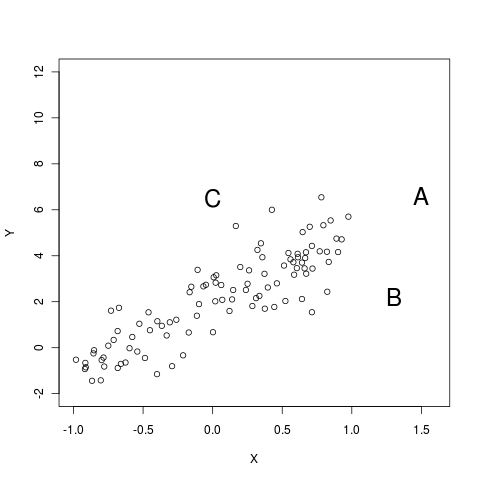
\includegraphics{leverage}}
\caption{Figure for Q. 3)}
  \end{figure}

  \begin{enumerate}
  \item Give a definition of {\em leverage}. 
Which of the labelled points ($A, B$ or $C$)
would you think have a high leverage value? Explain.
%A, B

\item Which of the labelled points ($A, B$ or $C$)
would you think would be labelled as an outlier by an outlier detection test? Explain.
% B or C

\item What does Cook's Distance try to measure for a multiple linear regression model? Which of the labelled points ($A, B$ or $C$)
would you think would have a large Cook's distance? Explain.
  \end{enumerate}
% B or C


\newpage 

\item Figure 2 shows the diagnostic plots from a model
fit predict {\tt MPG} (miles per gallon) of several makes of cars, based on {\tt WT} (weight), {\tt SP} (speed); {\tt VOL} (cab volume) and {\tt HP} (horse power).

  \begin{enumerate}
  \item Briefly describe the assumptions used in fitting this model. Do any of the assumptions seem to be violated based on Figure \ref{fig2}?
If any seem to be violated, suggest some possible fixes.


\item As part of the output, the researchers computed both a 95 \% confidence interval and a 95 \% prediction interval for the {\tt MPG} of a car with {\tt WT=30, HP=120, SP=110, VOL=100}, only they can't remember which of the following two intervals was which.
\begin{verbatim}
          fit      lwr      upr
[1,] 39.71459 37.56043 41.86874
>
          fit      lwr      upr
[1,] 39.71459 32.12874 47.30044
> 
\end{verbatim}
Which interval is the confidence interval? Explain.

\item Your friend now says:
  \begin{quote}
    {\em So this means that if you repeat this experiment
100 times, roughly 95 times the true mean weight of a car
with {\tt WT=30, HP=120, SP=110, VOL=100} will be between the limits
of the confidence interval you chose in (b) (either [32.1,47.3] or [37.5,41.9]).}
  \end{quote}
Do you agree? Why or why not?

  \item As part of this project, the researcher also wants to find
a model that fits the model possibly better than this current model. The researcher is willing to consider some potential
interactions in the model. Describe some possible approaches, being as explicit as reasonably possible (use {\tt R} pseudo-commands if you like).  

  \end{enumerate}


\begin{figure}
  \label{fig2}
  \centering
  \resizebox{!}{3.5in}{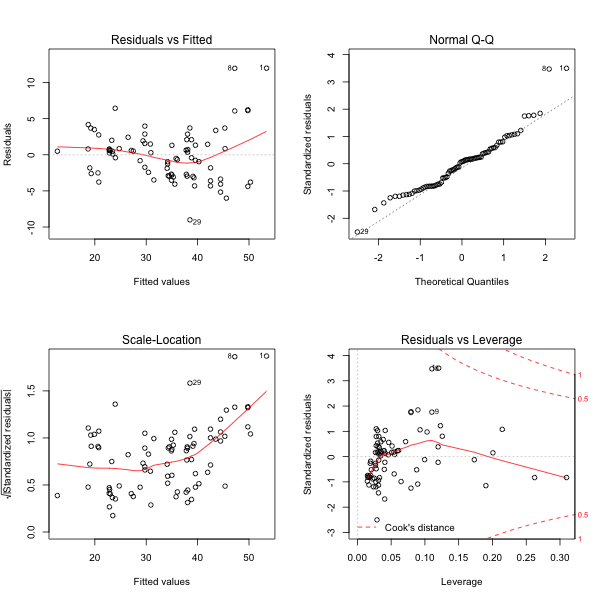
\includegraphics{mpg}}
\caption{Diagnostic plots for regression of MPG (miles per gallon) of several makes of cars, based on {\tt WT} (weight), {\tt SP} (speed); {\tt VOL} (cab volume) and {\tt HP} (horse power).}
\end{figure}

\newpage 

\item A liver specialist has come to you data relating 
the number of alcoholic beverages per week for each subject 
to 
the chances that they have develop liver disease (within some long
follow-up period). The study controlled for the effects of 
{\tt Age} as well as overall fitness level {\tt Fitness} with a high
value indicating a very fit subject. The results
of a logistic regression used in the study were:
\begin{verbatim}

Call:
glm(formula = Y ~ Age + Drinks + Fitness, family = binomial(link='logit'))

Deviance Residuals:
     Min        1Q    Median        3Q       Max
-1.21798  -0.26941  -0.16629  -0.08747   2.44946

Coefficients:
            Estimate Std. Error z value Pr(>|z|)
(Intercept)   2.8436     5.1508   0.552  0.58090
Age          -0.0993     0.1028  -0.966  0.33418
Drinks        0.1601     0.1208   1.325  0.18503
Fitness      -0.7584     0.2411  -3.146  0.00166 

\end{verbatim}

\begin{enumerate}

\item What is the estimated probability that a 50-year old who drinks
5 drinks a week of fitness level 3 will develop
liver disease? ({\sc If you don't have a calculator, just don't simplify the expression}).

\item Redo this calculation for a 50-year old of the same fitness level who does not drink any alcoholic beverages? ({\sc If you don't have a calculator, just don't simplify the expression}).


\item Using an odds ratio, approximate how many more times likely is the
adult who drinks 5 drinks likely to develop liver disease than the person who drinks none? 


\item Construct approximate Bonferroni-adjusted 90\% confidence intervals
for the coefficients of {\tt Age, Drinks, Fitness}. ({\sc See below for some potentially
useful {\tt R} output})

\end{enumerate}

\newpage

Some potentially useful {\tt R} output for Q. 4):

\begin{verbatim}
> qnorm(1-0.1)
[1] 1.281552
> qnorm(1-0.1/2)
[1] 1.644854
> qnorm(1-0.1/3)
[1] 1.833915
> qnorm(1-0.1/6)
[1] 2.128045
>                  
\end{verbatim}

\end{enumerate}

\end{document}




\begin{table}[htbp]
  \centering
  \begin{tabular}{ccc} \hline
Variable & Coefficient & SE  \\ \hline
Constant & 4.03 & 3.26  \\
Units & 15.21 & 0.52  \\ \hline
  \end{tabular}
  \caption{Regression Output When $Y$ is Regressed on $X$ for the computer repair data.}
  \label{tab:1}
\end{table}

For this question, use the following table, based on a regression for predicting the 
length of a service call at a computer repair company and the number of units
needing to be repaired. A total of $n=15$ calls were used to fit the model.

Test the following hypotheses at level $\alpha=0.1$.
\begin{enumerate}
\item $H_0: \beta_1=15$ vs. $H_1:\beta_1 \neq 15$

\item $H_0:\beta_1=15$ vs. $H_1:\beta_1 > 15$ 

\item $H_0:\beta_0=0$ vs. $H_1:\beta_0 \neq 0$ 

\item $H_0:\beta_0=5$ vs. $H_1:\beta_0 \neq 5$ 

\end{enumerate}

What are the assumptions you are making? 


\item A study is conducted to investigate the relationship
between LDL cholesterol (low-density lipoprotein), body
weight (W) and gender (G, 1=Male) in a certain population.
The data can be found at
\begin{quote}
\href{\homeurl/data/LDL.table}{\homeurl/data/LDL.table}  
\end{quote}

Answer the following questions, using $\alpha=0.05$ if not specified.
\begin{enumerate}
\item Is there a linear relationship between LDL and weight? 

\item Is the relationship the same within the male and female groups? If not, what is
different?

\item Use a model selection procedure to select a model that best describes the relationship between LDL, weight and gender in this population.
\end{enumerate}


\end{enumerate}



 \item Three types of fertilizer are to be tested to see
which one yields more corn crop. Forty similar plots of land were available
for testing purposes. The 40 plots are divided at random into four groups,
ten plots in each group. Fertilizer 1 was applied to each of the ten corn plots
in Group 1. Similarly, Fertilizers 2 and 3 were applied to the
plots in Groups 2 and 3, respectively. The corn plants in Group 4
were not given any fertilizer; it will serve as the control group.
The data can be found at
\begin{quote}
\href{\homeurl/data/yield.table}{\homeurl/data/yield.table}  
\end{quote}

Answer the following questions, using $\alpha=0.05$ if not specified.
\begin{enumerate}
\item With $Y_{ij}$ being the $j$-th observation in the $i$-th group,
fit a model
$$
Y_{ij} = \mu_i + \varepsilon_{ij}.
$$

\item Test the hypothesis that, on the average, none of the three
types of fertilizer has an effect on corn crops. Specify the hypothesis
to be tested, the test statistic and the results.

\item Test the hypothesis that, on the average, the three
types of fertilizer has the same effect on corn crops but different
than the control group 4. Specify the hypothesis
to be tested, the test statistic and the results.


\item Find Bonferroni simultaneous 90\% confidence intervals for the
mean yield in each of the four groups.
\end{enumerate}


\item 
\begin{table}[htbp]
  \centering
  \begin{tabular}{r|ll} 
&          Df & SSE  \\ \hline
Use &          2 &  33.24 \\
Size  &         3 &  12.06  \\
Size:Use &        6 &   4.25  \\
Residuals & 108 & 154.62 
  \end{tabular}
  \caption{ANOVA output for gasoline consumption analysis}
  \label{tab:3}
\end{table}

In order to determine some of the factors that effect
gasoline consumption, the fuel average miles per gallon for
 120 families and their cars were tracked over several months. The 
cars were categorized in to 4 categories: compact, sedan, minivan, SUV;
and the prevalent use was broken down into 3 categories: commuting to work, weekend, driving to school.
The sums of squares of a two-way analysis of variance (ANOVA)
model are presented above. 

\begin{enumerate}
\item What assumptions does the two-way ANOVA model make? Be precise as possible.

\item Test for the main effects of both Use and Size at level $\alpha=0.05$.
Does Use and / or  Size have an effect on average MPG?

\item Is there any significant interaction (at level $\alpha=0.05$) between 
Use and Size and their effect on average MPG?
\end{enumerate}

\item 
\begin{table}[htbp]
  \centering
  \begin{tabular}{c|ccccc} \hline
&  Contra Costa & Santa Clara & Los Angeles & San Bernadino \\ \hline
Yes   &  117	& 222 & 	 133 	& 109 	   \\
No &	404  &	334 	& 204  &	263   \\ \hline
  \end{tabular}
  \caption{Responses to earthquake insurance survey for Q. 4)}
  \label{tab:2}
\end{table}

A questionnaire was sent out to California homeowners asking whether or not
they had purchased earthquake insurance.

\begin{enumerate}
\item Test at level $\alpha=0.05$, using a Poisson regression model, whether the probability of having
earthquake insurance is the same in each county in the survey. What assumptions are you making in the model? What is the null hypothesis, $H_0$? The alternative $H_a$?


\item Also of interest is whether the probability of a homeowner having earthquake insurance is 50\% in
all counties. Translate the probability being 50\% into a statement
about the means in the Poisson model.
\item Test the hypothesis, at level $\alpha=0.05$ that the probability of having earthquake insurance is 50\% in each county surveyed.

\end{enumerate}

